\documentclass[border=6pt]{standalone}
\usepackage{tikz}
\usetikzlibrary{arrows.meta,positioning,calc,shapes.geometric,fit,backgrounds,patterns,matrix,decorations.pathreplacing}
\begin{document}
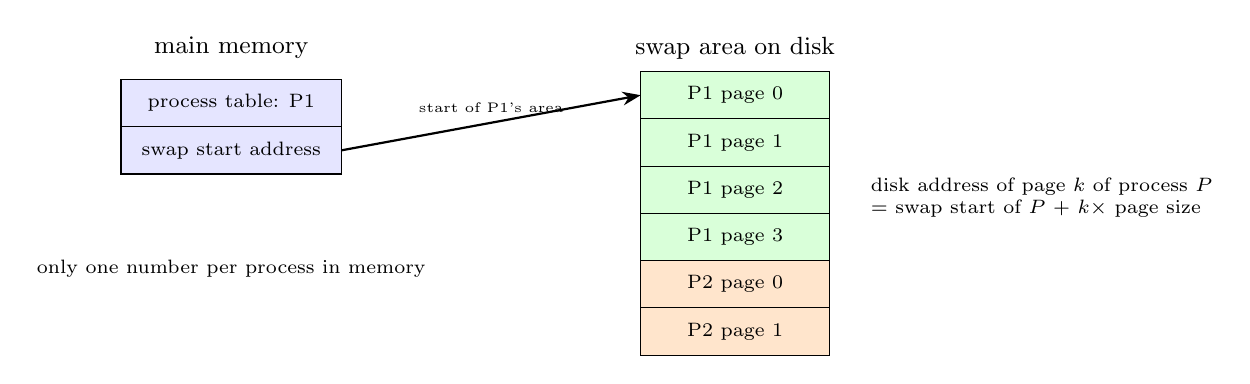
\begin{tikzpicture}[>=Stealth,font=\small]
\tikzstyle{b}=[draw,minimum height=0.6cm,font=\scriptsize]
\node[font=\small] at (1.2,2.2) {main memory};
\node[b,fill=blue!10,minimum width=2.8cm] at (1.2,1.5) {process table: P1};
\node[b,fill=blue!10,minimum width=2.8cm] at (1.2,0.9) {swap start address};
\node[font=\small] at (7.6,2.2) {swap area on disk};
\foreach \i/\t in {0/{P1 page 0},1/{P1 page 1},2/{P1 page 2},3/{P1 page 3},4/{P2 page 0},5/{P2 page 1}} \node[b,minimum width=2.4cm,fill=\ifnum\i<4 green!15\else orange!20\fi] at (7.6,1.6-\i*0.6) {\t};
\draw[->,thick] (2.6,0.9) -- (6.4,1.6) node[midway,above,font=\tiny]{start of P1's area};
\node[font=\scriptsize,align=left,anchor=west] at (9.2,0.3) {disk address of page $k$ of process $P$\\ $=$ swap start of $P$ $+$ $k\times$ page size};
\node[font=\scriptsize,align=left] at (1.2,-0.6) {only one number per process in memory};
\end{tikzpicture}
\end{document}
